\section{Wyniki eksperymentów symulacyjnych}
\begin{frame}
\frametitle{\secname}
\framesubtitle{Otwarta przestrzeń ustawienie prostopadłe}
	\begin{figure}[ht] % h:here; t:top; b:bottom; p:page; default:ht
		\centering
			\captionsetup[subfigure]{labelformat=empty}
			\centering
			\subfloat[][1-2]
			{
				\includegraphics[page = 2, width=0.49\textwidth]{img/Simulation_Open_space.pdf}
			}
			\subfloat[][10-9]
			{
				\includegraphics[page = 99, width=0.49\textwidth]{img/Simulation_Open_space.pdf}
			}
\end{figure}
\end{frame}

\section*{Wyniki eksperymentów symulacyjnych}
\begin{frame}
\frametitle{\secname}
\framesubtitle{Przejście przez drzwi}
\begin{figure}[ht] % h:here; t:top; b:bottom; p:page; default:ht
		\captionsetup[subfigure]{labelformat=empty}
		\centering
		\subfloat[][1-H2]
		{
			\includegraphics[page = 2, width=0.49\textwidth]{img/Simulation_Passage_through_the_door.pdf}
		}
		\subfloat[][9-H8]
		{
			\includegraphics[page = 88, width=0.49\textwidth]{img/Simulation_Passage_through_the_door.pdf}
		}
\end{figure}
\end{frame}

\section*{Wyniki eksperymentów symulacyjnych}
\begin{frame}
\frametitle{\secname}
\framesubtitle{Wąski korytarz}

\begin{figure}[ht] % h:here; t:top; b:bottom; p:page; default:ht
	\captionsetup[subfigure]{labelformat=empty}
	\centering
	\subfloat[][8-3]
	{
		\includegraphics[page = 73, width=0.6\textwidth]{img/Simulation_A_narrow_corridor.pdf}
	}
\end{figure}
\end{frame}

\section*{Eksperyment na rzeczywistych robotach}
\begin{frame}
\frametitle{\secname}

\begin{itemize}
	\item Obudowa A4WD1v2 Lynxmotion 22cm x 20cm x 6cm.
	\item Zasilanie dwie baterie litowo-polimerowe o nominalnym napięciu 14.8V i pojemności 5Ah.
	\item Sterowniki silników RoboClaw 2 x 15A firmy BasicMicro.
	\item Komputer sterujący PandaBoard ES:	
	\begin{itemize}
		\item dwurdzeniowy procesor Cortex-A9 OMAP4460 taktowany zegarem 1,2 GHz,
		\item RAM 1GB,
		\item Ethernet RJ45 100Mb,
		\item WiFi 802.11 b/g/n i Bluetooth 2.1,
		\item USB 2.0,
		\item I2C,
		\item SPI.
	\end{itemize}
	\item Skaner laserowy URG-04LX-UG01 firmy Hokuyo.	
\end{itemize}

\begin{textblock*}{4cm}(8.5cm,5.2cm) % {block width} (coords)
	\includegraphics[page=1,width=4cm]{img/Rysunki.pdf}
\end{textblock*}
\tiny{
	Open Source Hardware \\
	Strona projektu: \url{http://capo.iisg.agh.edu.pl/}}

\note{W celu zweryfikowania poprawności działania algorytmów wykorzystano platformę CAPO zbudowaną na AGH.}
\end{frame}

\section{Wyniki eksperymentów z wykorzystaniem rzeczywistych robotów}
\begin{frame}
\frametitle{\secname}
\framesubtitle{Otwarta przestrzeń ustawienie prostopadłe}
\begin{figure}[ht] % h:here; t:top; b:bottom; p:page; default:ht
	\captionsetup[subfigure]{labelformat=empty}
	\centering
	\subfloat[][1-2]
	{
		\includegraphics[page = 2, width=0.6\textwidth]{img/Robots_Open_space.pdf}
	}
\end{figure}
\end{frame}

\section*{Wyniki eksperymentów z wykorzystaniem  rzeczywistych robotów}
\begin{frame}
\frametitle{\secname}
\framesubtitle{Przejście przez drzwi}
\begin{figure}[ht] % h:here; t:top; b:bottom; p:page; default:ht
	\captionsetup[subfigure]{labelformat=empty}
	\centering
	\subfloat[][1-H2]
	{
		\includegraphics[page = 2, width=0.6\textwidth]{img/Robots_Passage_through_the_door.pdf}
	}
\end{figure}
\end{frame}